\chapter{Решаем задачи в функциональном стиле}
\label{functionally-solving-problems}
\colorbox{lgray}
{
\begin{minipage}{1.0\linewidth}
    Похоже, что мы уже выпили достаточно эрлангового сока, чтобы создать что\--нибудь полезное.
    В этой главе не будет нового материала.
    Я просто покажу как применять элементы увиденного ранее.
    Задачи были взяты из книги Miran\--а \href{http://learnyouahaskell.com/functionally-solving-problems}{Learn You a Haskell}.
    Для всех примеров я использовал аналогичный способ решения, чтобы любопытный читатель смог сравнивать код на Erlang и Haskell как ему заблагорассудится.
    Проведя такое сравнение, вы, наверняка, придёте к заключению, что для двух языков с очень разными синтаксисами, решения очень похожи друг на друга.
    Это сходство обусловлено тем, что изученные концепции функционального программирования можно сравнительно легко переносить на другие функциональные языки.
\end{minipage}
}
\section{Калькулятор в обратной польской записи}
\label{reverse-polish-notation-calculator}
Большинство людей обучены записи арифметических выражений, согласно которой оператор помещают между чисел (\ops{(2 + 2) / 5}).
Так вводятся математические выражения в большинстве калькуляторов, и, скорее всего,  такую запись вас обучили использовать при счёте на школьных уроках. 
У этой записи есть недостаток: вам необходимо знать порядок вычисления операторов.
Умножение и деление считается более важным (имеет более высокий приоритет), чем сложение и вычитание.

Существует ещё один способ записи, который называется \emph{префиксной записью} или \emph{польской записью}, в которой оператор записывается перед операндами.
В этой записи выражение \ops{(2 + 2) / 5} примет вид \ops{(/ (+ 2 2) 5)}.
Если мы решим, что \ops{+\strut}  и \ops{/\strut} должны всегда принимать два аргумента, то \ops{(/ (+ 2 2) 5)} можно просто записать как \ops{/ + 2 2 5}.

Однако, мы сосредоточимся на \emph{обратной польской записи} (или просто ОПЗ), которая противоположна префиксной записи: в ней оператор следует за операндами.
Тот же самый пример, приведённый выше, в ОПЗ будет записан как \ops{2 2 + 5 /}.
Можно привести и другие примеры: \ops{9 * 5 + 7} и \ops{10 * 2 * (3 + 5) / 2} транслируются соответственно в \ops{9 5 * 7} и \ops{10 2 * 3 4 + * 2 /}.
Эта запись очень широко использовалась в ранних моделях калькуляторов, так как экономно использует память.
А некоторые люди до сих пор таскают с собой калькуляторы с ОПЗ.
Именно такой калькулятор мы и напишем.

Для начала, неплохо было бы понимать, как читаются выражения ОПЗ.
Первый способ: по одному находим операторы и, учитывая арность, группируем их с операндами.
\begin{align*}
    &10\;4\;3+2 * -\\
    &10\;(4\;3\; +)\;2 * -\\
    &10\; ((4\; 3\; +)\; 2\; *) -\\ 
    &(10\; ((4\; 3\; +)\; 2\; *) -)\\
    &(10\; (7\; 2\; *) -)\\
    &(10\; 14\; -)\\
    &-4\\
\end{align*}

Однако, в компьютере или калькуляторе намного проще создать \emph{стек} всех операндов в порядке их расположения.
Возьмём математическое выражение \ops{10 4 3 + 2 * -}.
Первый операнд 10.
Мы добавляем его в стек.
Затем идёт 4.
Его мы тоже кладём на вершину стека.
Третьим идёт число 3.
Мы помещаем в стек и его.
Теперь стек принял следующий вид:
\begin{figure}[h!]
    \centering
    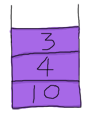
\includegraphics[width=0.12\textwidth]{stack1.png}
\end{figure}

Следующий символ это \ops{+\strut}.
Он представляет собой функцию арности 2.
Чтобы ею воспользоваться, нам необходимо передать ей два операнда, которые мы извлечём из стека:
\begin{figure}[h!]
    \centering
    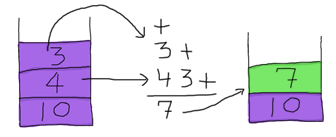
\includegraphics[width=0.4\textwidth]{stack2.png}
\end{figure}

Полученную цифру 7 мы загоняем в верхушку стека (фу, мы же не хотим, чтобы эти грязные числа шатались повсюду!)
Теперь стек содержит [7, 10], и от первоначального выражения осталось лишь \ops{2 * -}.
Мы берём 2 и помещаем его в вершину стека.
Затем мы видим операцию \ops{*\strut}, которой для работы необходимо передать два операнда.
И снова мы извлекаем их из стека:
\begin{figure}[h!]
    \centering
    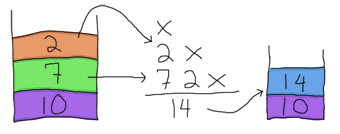
\includegraphics[width=0.4\textwidth]{stack3.png}
\end{figure}

И помещаем 14 в вершину стека.
Остаётся лишь \ops{-\strut}, которому необходимо передать два операнда.
Невероятная удача!
В стеке как раз осталось два операнда.
Пустим их в дело!
\begin{figure}[h!]
    \centering
    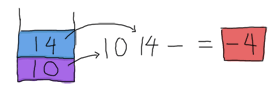
\includegraphics[width=0.4\textwidth]{stack4.png}
\end{figure}

Ну вот мы и получили результат.
Этот стек\--ориентированный подход сравнительно надёжен.
Тот факт, что для начала вычислений требуется разбирать мало данных, объясняет почему этот способ годится даже для старых калькуляторов.
ОПЗ стоит использовать и по другим причинам, но их обсуждение выходит за рамки этого руководства..
Заинтересовавшимся лучше обратиться к \href{http://en.wikipedia.org/wiki/Reverse_Polish_notation}{статье на Wikipedia}.

Как только мы справились со сложными моментами, записать решение на Erlang становится достаточно просто.
Оказывается, самое сложное \--- определить шаги для получения конечного результата.
А это мы только что проделали.
Неплохо.
Откройте файл \emph{\href{http://learnyousomeerlang.com/static/erlang/calc.erl}{calc.erl}}.

Для начала озаботимся представлением математических выражений.
Чтобы упростить задачу мы, наверное, представим их в виде строки: \ops{''10 4 3 + 2 * -''}.
В этой строке между термами есть пробелы, которые не оговорены в нашем решении, но для работы простого лексического анализатора они необходимы.
После обработки входящей строки анализатором, мы ожидаем получить список термов вида \ops{[''10'',''4'',''3'',''+'',''2'',''*'',''-'']}.
Оказывается, функция \ops{\href{http://erldocs.com/R15B/stdlib/string.html\#tokens/2}{string:tokens/2}} делает именно то, что нам нужно:
\begin{lstlisting}[style=erlang]
1> string:tokens("10 4 3 + 2 * -", " ").
["10","4","3","+","2","*","-"]
\end{lstlisting}

Такое представление выражения нам подойдёт.
Следующим шагом мы должны определить стек.
Как мы это сделаем?
Возможно, вы заметили, что поведение списков в Erlang очень похоже на стек.
Оператор (\ops{|}) в шаблоне \ops{[Head|Tail]} ведёт себя так же как и операция добавления \emph{Head} в вершину стека (которой в данном случае является \emph{Tail}).
Список в роли стека нам вполне подойдёт.

Чтобы прочитать выражение, нам необходимо просто повторить те же действия, которые мы выполняли при решении задачи вручную.
Последовательно считываем каждое значение в выражении.
Если мы прочитали число \--- кладём его на стек.
Если функцию \--- извлекаем все необходимые ей значения из стека, а результат вычисления возвращаем обратно в стек.
Если обобщить задачу, то нам нужно один раз пройти в цикле по всему выражению и по ходу движения накапливать результаты.
С этим прекрасно справится свёртка (fold)!

Теперь мы должны выяснить, как будет выглядеть функция, которую \ops{\href{http://erldocs.com/R15B/stdlib/lists.html\#foldl/3}{lists:foldl/3}} будет применять к каждому оператору и операнду в нашем выражении.
Функция будет запускаться в свёртке, следовательно она должна принимать два аргумента: первый будет содержать элемент выражения, который будет обрабатывать функция, а вторым будет передаваться стек.

Начнём редактировать наш код в файле \ops{\href{http://learnyousomeerlang.com/static/erlang/calc.erl}{calc.erl}}.
Напишем функцию, в которой будет происходить итерация, а также удаление пробелов из выражения:
\begin{lstlisting}[style=erlang]
-module(calc).
-export([rpn/1]).
 
rpn(L) when is_list(L) ->
    [Res] = lists:foldl(fun rpn/2, [], string:tokens(L, " ")),
    Res.
\end{lstlisting}

Следующим шагом реализуем функцию \ops{rpn/2}.
Обратите внимание: каждый оператор и операнд из выражения в конце концов попадает на вершину стека, а поэтому и конечный результат вычислений также окажется в стеке.
Мы извлекаем последнее значение из стека и возвращаем его пользователю.
Именно поэтому в сопоставлении с образцом мы используем шаблон \ops{[Res]} и возвращаем \emph{Res}.

Хорошо, а теперь более сложный момент.
Наша функция \ops{rpn/2} должна обрабатывать стек для всех переданных ей значений.
Заголовок функции, скорее всего, будет выглядеть как \ops{rpn(Op,Stack)}, а возвращаемое значение примет вид \ops{[NewVal|Stack]}.
Для обычных чисел будет выполняться операция:
\begin{lstlisting}[style=erlang]
rpn(X, Stack) -> [read(X)|Stack].
\end{lstlisting}

Функция \ops{read/1} конвертирует строку в целое число или число с плавающей точкой.
К сожалению, в Erlang нет встроенной функции, которая делает и то и другое, поэтому мы создадим её сами:
\begin{lstlisting}[style=erlang]
read(N) ->
    case string:to_float(N) of
        {error,no_float} -> list_to_integer(N);
        {F,_} -> F
    end.
\end{lstlisting}

Где \ops{\href{http://erldocs.com/R15B/stdlib/string.html\#to\_float/1}{string:to\_float/1}} производит конвертацию строк вида ''13.37'' в их числовой эквивалент.
Если значение числа с плавающей запятой определить не удаётся, функция возвращает \ops{\{error,no\_float\}}.
После чего мы должны вызвать функцию \ops{list\_to\_integer/1}.

А теперь снова вернёмся к \ops{rpn/2}.
Все найденные числа мы отправляем в стек.
Но так как наше сопоставление с образцом захватывает любые значения (см. \ref{pattern-matching}), то кроме чисел в стек также будут попадать и операторы.
Чтобы этого избежать, мы добавим для всех операторов конкретные шаблоны, которые будут предварять общий.
Начнём со сложения:
\begin{lstlisting}[style=erlang]
rpn("+", [N1,N2|S]) -> [N2+N1|S];
rpn(X, Stack) -> [read(X)|Stack].
\end{lstlisting}

Очевидно, что каждый раз когда нам попадается строка \ops{''+''}, мы извлекаем из стека два числа \emph{(N1,N2)}, складываем их и возвращаем результат в стек.
Именно такие действия мы выполняли, когда решали задачу вручную.
Запустив программу, мы можем убедиться в её работоспособности:
\begin{lstlisting}[style=erlang]
1> c(calc).
{ok,calc}
2> calc:rpn("3 5 +").
8
3> calc:rpn("7 3 + 5 +").
15
\end{lstlisting}

Остальное \--- тривиально.
Нужно  лишь добавить такие же строки для всех оставшихся  операторов:
\begin{lstlisting}[style=erlang]
rpn("+", [N1,N2|S]) -> [N2+N1|S];
rpn("-", [N1,N2|S]) -> [N2-N1|S];
rpn("*", [N1,N2|S]) -> [N2*N1|S];
rpn("/", [N1,N2|S]) -> [N2/N1|S];
rpn("^", [N1,N2|S]) -> [math:pow(N2,N1)|S];
rpn("ln", [N|S])    -> [math:log(N)|S];
rpn("log10", [N|S]) -> [math:log10(N)|S];
rpn(X, Stack) -> [read(X)|Stack].
\end{lstlisting}

Обратите внимание, что функции, которые принимают лишь один аргумент (например функция логарифмирования), должны извлекать из стека один элемент.
Пусть читатель в качестве упражнения добавит функции 'sum' или 'prod', которые, соответственно, возвращают сумму и произведение всех считанных элементов.
Если у вас возникнут затруднения, обратитесь к моей реализации этих функций в \ops{\href{http://learnyousomeerlang.com/static/erlang/calc.erl}{calc.erl}}.

Мы напишем несколько простых юнит\--тестов, чтобы убедиться, что всё работает как положено.
Оператор \ops{=\strut} в Erlang можно использовать как функцию \emph{утверждения (assertion)}.
Если после проверки утверждения обнаружены значения, которые ему не соответствуют \--- должен происходить сбой.
Это как раз то, что нам нужно.
Конечно, в Erlang есть и более совершенные тестовые фреймворки, например \href{http://erlang.org/doc/apps/common_test/write_test_chapter.html}{Common Test} и \href{http://erlang.org/doc/apps/eunit/chapter.html}{EUnit}.
Мы поговорим о них позже, а сейчас нам хватит и \ops{=\strut}.
\begin{lstlisting}[style=erlang]
rpn_test() ->
    5 = rpn("2 3 +"),
    87 = rpn("90 3 -"),
    -4 = rpn("10 4 3 + 2 * -"),
    -2.0 = rpn("10 4 3 + 2 * - 2 /"),
    ok = try
        rpn("90 34 12 33 55 66 + * - +")
    catch
        error:{badmatch,[_|_]} -> ok
    end,
    4037 = rpn("90 34 12 33 55 66 + * - + -"),
    8.0 = rpn("2 3 ^"),
    true = math:sqrt(2) == rpn("2 0.5 ^"),
    true = math:log(2.7) == rpn("2.7 ln"),
    true = math:log10(2.7) == rpn("2.7 log10"),
    50 = rpn("10 10 10 20 sum"),
    10.0 = rpn("10 10 10 20 sum 5 /"),
    1000.0 = rpn("10 10 20 0.5 prod"),
    ok.
\end{lstlisting}

Тестовая функция пытается исполнить все операции.
Тест считается пройденным, если не было возбуждено исключение.
Четыре первых теста проверяют корректную работу арифметических функций.
Пятый тест задаёт поведение, которое я пока ещё не обсуждал.
Выражение \ops{try \ldots catch} ожидает, что будет брошена ошибка badmatch, так как выражение невозможно вычислить:
\begin{lstlisting}[style=erlang]
90 34 12 33 55 66 + * - +
90 (34 (12 (33 (55 66 +) *) -) +)
\end{lstlisting}

Под конец выполнения функции \ops{rpn/1} значения -3947 и 90 остаются в стеке, так как не хватает оператора, который бы произвёл действие над числом 90.
Эта проблема имеет два решения: её можно проигнорировать и просто взять значение, которое находится на вершине стека (это будет последний вычисленный результат), или сгенерировать ошибку, которая сообщит о неверных арифметических действиях.
Так как политика Erlang для таких случаев требует, чтобы мы позволили процессу упасть, то мы в этой ситуации сделаем выбор в пользу именно этого требования.
Сбой происходит в шаблоне \ops{[Res]} функции \ops{rpn/1}.
Шаблон проверяет, что в стеке остался лишь один элемент, и этот элемент \--- конечный результат вычислений.

Несколько тестов вида \ops{true = FunctionCall1 == FunctionCall2} были добавлены, так как по левую сторону от \ops{=\strut} нельзя использовать вызов функции.
Но они всё равно работают аналогично утверждениям, потому что мы сравниваем результат сравнения с \emph{true}.

Также я добавил тесты для операторов sum и prod, чтобы вы смогли поупражняться в их реализации.
Если все тесты прошли успешно, то вы должны увидеть следующее:
\begin{lstlisting}[style=erlang]
1> c(calc).
{ok,calc}
2> calc:rpn_test().
ok
3> calc:rpn("1 2 ^ 2 2 ^ 3 2 ^ 4 2 ^ sum 2 -").
28.0
\end{lstlisting}

Где число 28 действительно равно результату вычисления \ops{$sum(1^2 + 2^2 + 3^2 + 4^2) - 2$}.

Наш калькулятор можно улучшить, добавив возбуждение исключений \ops{badarith} в случае аварийного завершения из\--за неизвестных операторов или из\--за оставленных на стеке необработанных значений.
Такое исключение обозначает проблему чётче, чем ошибка \ops{badmatch}, которую мы генерируем сейчас.
Этим мы значительно облегчим отладку для пользователя модуля calc.

\section{Из Хитроу в Лондон}
\label{heathrow-to-london}
Следующая задача также взята из \href{http://learnyouahaskell.com/functionally-solving-problems#heathrow-to-london}{Learn You a Haskell}.
Вы летите в самолёте, который через несколько часов должен приземлиться в аэропорте Хитроу.
После приземления необходимо как можно быстрее добраться до Лондона.
Ваш богатый дядя при смерти, и вы хотите первым предъявить права на его недвижимость.

Из Хитроу в Лондон проложены две дороги, которые сообщаются при помощи нескольких переулков.
Некоторые части дорог и переулков, из\--за скоростных ограничений и заторов, позволяют ехать медленнее, чем другие.
Перед посадкой вы решаете найти оптимальный путь, ведущий к дому, и, тем самым, максимизировать свои шансы.
Вот карта, которую вы нашли при помощи своего лэптопа:
\begin{figure}[h!]
    \centering
    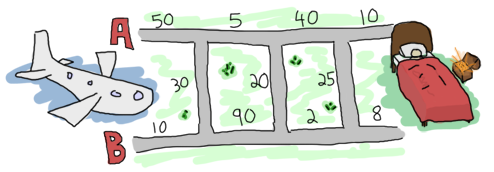
\includegraphics[width=0.7\textwidth]{road1.png}
\end{figure}

Так как после прочтения нескольких онлайн\--книг вы стали ярым фанатом Erlang\--а, то, конечно же, хотите решить эту задачу на вашем любимом языке.
Чтобы облегчить работу с картой, вы сохраняете исходные данные в файле \href{http://learnyousomeerlang.com/static/erlang/road.txt}{road.txt} следующим образом:
\begin{lstlisting}[style=erlang]
50
10
30
5
90
20
40
2
25
10
8
0
\end{lstlisting}

Информация о дороге организована по шаблону:
\ops{A1, B1, X1, A2, B2, X2, ..., An, Bn, Xn}, где \emph{x} \--- это один из переулков, соединяющих между собой части А и B.
В качестве последнего сегмента \emph{x} мы используем 0, так как в этот момент мы гарантированно будем находиться в пункте назначения.
Данные можно организовать в кортежи по 3 элемента (тройки) вида \ops{\{A,B,X\}}.

И тут вы понимаете, что если вы не знаете как решить эту задачу вручную, то нечего даже пытаться решить её на Erlang.
Для анализа задачи будем использовать то, чему нас научила рекурсия.

Первым шагом мы пытаемся найти частный случай.
Для нашей задачи это ситуация, когда осталось проанализировать лишь один кортеж.
То есть, сделать выбор между \emph{A, B} (и переулком \emph{x}, который в данном случае бесполезен, так как мы находимся в пункте назначения):
\begin{figure}[h!]
    \centering
    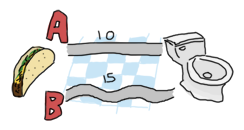
\includegraphics[width=0.5\textwidth]{road2.png}
\end{figure}

Поэтому остаётся лишь определить, какой путь короче \--- путь A или путь B.
Если вы хорошо изучили рекурсию, то знаете, что мы обязаны сходиться к частному случаю, то есть, на каждом шаге мы будем пытаться свести задачу к выбору между A и B.

Расширим нашу карту и начнём заново:
\begin{figure}[h!]
    \centering
    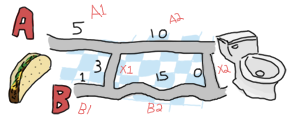
\includegraphics[width=0.5\textwidth]{road3.png}
\end{figure}

О, это уже интереснее!
Как мы можем перейти от тройки \ops{\{5,1,3\}} к чёткому выбору между A и B?
Определим, сколько существует вариантов для A.
Чтобы добраться до пересечения \emph{A1} и \emph{A2} (я буду называть это место \emph{точкой A1}), я могу поехать напрямую по дороге \emph{A1} (5), либо проехать по \emph{B1} (1), а затем по переулку \emph{X1} (3).
В этом случае первый вариант (5) длиннее второго (4).
Кратчайший путь для варианта А это \ops{[B, X]}.
А какие есть варианты для B?
Можно проехать по \emph{A1} (5), затем по переулку \emph{X1} (3), или сразу же избрать путь \emph{B1} (1).

Хорошо!
У нас есть путь длины 4 \ops{[B, X]} до первого пересечения А, и путь длины 1 \ops{[B]} до пересечения \emph{B1} и \emph{B2}.
Теперь мы должны сделать выбор между второй точкой A (пересечение \emph{A2} и конечной точки \emph{X2}) и второй точкой B (пересечение \emph{B2} и \emph{X2}).
Предлагаю сделать то же самое, что и раньше.
Так как тексты здесь пишу я, то моё решение вам оспорить не удастся.
Ну что ж, продолжим!

Все возможные пути для этого случая можно найти таким же способом, как и в предыдущей ситуации.
До точки A мы можем добраться либо по пути \emph{A2} из \ops{[B, X]}, который даёт нам длину 14 (\ops{14 = 4 + 10}, либо по \emph{B2}, а затем \emph{X2} из точки \ops{[B]}, что даёт нам длину 16 (\ops{16 = 1 + 15 + 0}).
Очевидно, что путь \ops{[B, X, A]} лучше пути \ops{[B, B, X]}.
\begin{figure}[h!]
    \centering
    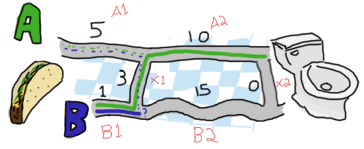
\includegraphics[width=0.7\textwidth]{road3_2.png}
\end{figure}

Также мы можем добраться до следующей точки B по пути \emph{A2} из \ops{[B, X]} и переулку \emph{X2}, что даст нам длину 14 (\ops{14 = 4 + 10 + 0}).
Либо по дороге \emph{B2} из \emph{[B]}, которая даст нам путь длины 16 (\ops{16 = 1 + 15}).
Мы выберем первый вариант: \ops{[B, X, A, X]}.

В конце у нас остаются два пути A и B.
Длина обоих равна 14.
Любой из этих маршрутов можно считать верным.
Окончательный  выбор всегда будет происходить между двумя маршрутами равной длины, если последний сегмент X имеет длину 0.
Наше рекурсивное решение даёт уверенность, что на выходе мы всегда получаем кратчайший путь.
Совсем неплохо, согласитесь.

Постепенно мы снабдили себя основными деталями, необходимыми для постройки рекурсивной функции.
Можете, конечно, её реализовать, если хотите, но я пообещал, что самостоятельно рекурсивные функции мы будем писать очень редко.
Здесь мы задействуем свёртку (fold).\\
\colorbox{lgray}
{
\begin{minipage}{1.0\linewidth}
    \textbf{Замечание:} хоть я и показывал, что свёртки используются для списков и создаются с их помощью, но свёртки представляют собой более универсальную концепцию перебора элементов структуры данных при помощи аккумулятора.
Поэтому свёртки можно реализовывать над деревьями, словарями (dictionaries), массивами, таблицами баз данных и т.д.

Во время экспериментов зачастую полезно использовать отображения (maps) и свёртки (folds).
С их помощью можно впоследствии легко изменить структуру данных, с которой работает логика вашей программы.
\end{minipage}
}

Итак, на чём мы остановились?
Ах, да!
Мы подготовили файл, который будем использовать как вход для нашей программы.
Для файловых манипуляций лучшим инструментом является \href{http://erldocs.com/R15B/kernel/file.html}{файловый модуль}.
Он содержит множество функций, которые встречаются в большинстве языков программирования и используются для работы с файлами (установка прав доступа, перемещение файлов, переименование и удаление и т.д.)

Модуль также содержит стандартные функции для чтения и/или записи из/в файлы, такие как \ops{\href{http://erldocs.com/R15B/kernel/file.html\#open/2}{file:open/2}} и \ops{\href{http://erldocs.com/R15B/kernel/file.html\#close/1}{file:close/1}}, которые делают именно то, о чём сообщают их имена (открывают и закрывают файлы!)
\ops{\href{http://erldocs.com/R15B/kernel/file.html\#read/2}{file:read/2}} извлекает из файла содержимое (в двоичном виде или в виде строки), \ops{\href{http://erldocs.com/R15B/kernel/file.html\#read\_line/1}{file:read\_line/1}} считывает единичную строку, \ops{\href{http://erldocs.com/R15B/kernel/file.html\#position/3}{file:position/3}} перемещает указатель в открытом файле в указанную позицию и т.д.

В модуле есть и несколько упрощённых функций, например \ops{\href{http://erldocs.com/R15B/kernel/file.html\#read\_file/1}{file:read\_file/1}} (открывает файл и читает его содержимое в двоичном виде), \ops{\href{http://erldocs.com/R15B/kernel/file.html\#consult/1}{file:consult/1}} (открывает и разбирает файл на термы Erlang) или \ops{\href{http://erldocs.com/R15B/kernel/file.html\#pread/2}{file:pread/2}} (меняет текущую позицию в файле, а потом считывает данные) и \ops{\href{http://erldocs.com/R15B/kernel/file.html\#pwrite/2}{pwrite/2}} (меняет текущую позицию и записывает данные).

С таким богатым выбором мы легко найдём функцию, которая позволит считать наш файл \href{http://learnyousomeerlang.com/static/erlang/road.txt}{road.txt}.
Так как нам известно, что описание дороги относительно невелико, то мы воспользуемся вызовом \ops{file:read\_file("road.txt").}:
\begin{lstlisting}[style=erlang]
1> {ok, Binary} = file:read_file("road.txt").
{ok,<<"50\r\n10\r\n30\r\n5\r\n90\r\n20\r\n40\r\n2\r\n25\r\n10\r\n8\r\n0\r\n">>}
2> S = string:tokens(binary_to_list(Binary), "\r\n\t ").
["50","10","30","5","90","20","40","2","25","10","8","0"]
\end{lstlisting}

Обратите внимание, что в данном случае я добавил пробел (\ops{'' ''\strut}) и символ табуляции (\ops{''\textbackslash t''}) в список валидных токенов, чтобы иметь возможность считывать файлы вида "50 10 30 5 90 20 40 2 25 10 8 0".
После считывания этого списка, нам нужно преобразовать строки в целые числа.
Применим способ, подобный тому, который мы использовали в нашем ОПЗ калькуляторе:
\begin{lstlisting}[style=erlang]
3> [list_to_integer(X) || X <- S].
[50,10,30,5,90,20,40,2,25,10,8,0]
\end{lstlisting}

Давайте создадим новый модуль, назовём его \href{http://learnyousomeerlang.com/static/erlang/road.erl}{road.erl} и запишем наши рассуждения в виде кода:
\begin{lstlisting}[style=erlang]
-module(road).
-compile(export_all).
 
main() ->
    File = "road.txt",
    {ok, Bin} = file:read_file(File),
    parse_map(Bin).
 
parse_map(Bin) when is_binary(Bin) ->
    parse_map(binary_to_list(Bin));
parse_map(Str) when is_list(Str) ->
    [list_to_integer(X) || X <- string:tokens(Str,"\r\n\t ")].
\end{lstlisting}

Функция \ops{main/0} отвечает за чтение содержимого файла и его передачу в функцию \ops{parse\_map/1}.
Так как для чтения мы используем функцию \ops{file:read\_file/1}, то полученный результат будет представлен в виде двоичных данных.
Поэтому я сделал так, чтобы функция \ops{parse\_map/1} проводила сопоставление и для списков, и для двоичных данных.
В случае двоичных данных мы просто повторно вызываем функцию и передаём ей строку, преобразованную в список (наша функция для разбиения строк работает только со списками).

Следующим шагом разбора данных, описывающих карту, будет перегруппировка чисел в кортежи \ops{\{A,B,X\}}, описанные ранее.
К сожалению, простого универсального способа выбрать из списка по 3 элемента за раз не существует, а поэтому нам придётся использовать сопоставление с образцом в рекурсивной функции:
\begin{lstlisting}[style=erlang]
group_vals([], Acc) ->
    lists:reverse(Acc);
group_vals([A,B,X|Rest], Acc) ->
    group_vals(Rest, [{A,B,X} | Acc]).
\end{lstlisting}

Эта функция оптимизируется в хвостовую рекурсию и ничего особенно сложного в ней не происходит.
Её нужно будет вызвать из слегка модифицированной функции \ops{parse\_map/1}:
\begin{lstlisting}[style=erlang]
parse_map(Bin) when is_binary(Bin) ->
    parse_map(binary_to_list(Bin));
parse_map(Str) when is_list(Str) ->
    Values = [list_to_integer(X) || X <- string:tokens(Str,"\r\n\t ")],
    group_vals(Values, []).
\end{lstlisting}

Если мы попробуем скомпилировать всё вместе, то получим осмысленное описание дороги:
\begin{lstlisting}[style=erlang]
1> c(road).
{ok,road}
2> road:main().
[{50,10,30},{5,90,20},{40,2,25},{10,8,0}]
\end{lstlisting}

Ага, похоже всё верно.
У нас появился ещё один элемент функции, которая потом попадёт в свёртку.
Теперь для осуществления задуманного нам нужен хороший аккумулятор.

Для выбора аккумулятора я использую следующий метод: представляю, что я внутри запущенного алгоритма.
Для этой конкретной задачи я представлю, что пытаюсь определить кратчайший путь для второй тройки (\ops{\{5,90,20\}}).
Чтобы определить лучший маршрут, мне нужно владеть результатом для предыдущей тройки.
К счастью, способ решения этой задачи нам уже известен, так как для него нам не понадобится аккумулятор, и всю необходимую логику мы уже записали.
Итак, для A:
\begin{figure}[h!]
    \centering
    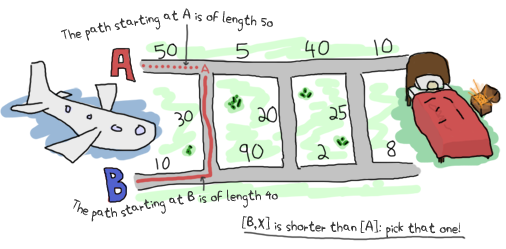
\includegraphics[width=0.85\textwidth]{road1_2.png}
\end{figure}

И из этих двух путей выбираем кратчайший.
\clearpage
Для B задача имеет похожее решение:
\begin{figure}[!htbp]
    \centering
    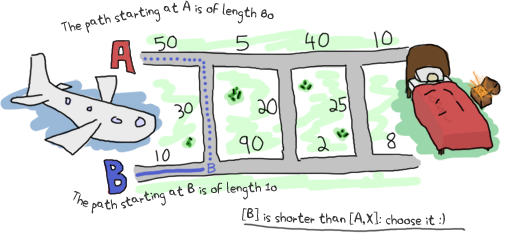
\includegraphics[width=0.85\textwidth]{road1_3.png}
\end{figure}

Теперь нам известно, что лучший путь в A на текущий момент \--- это \ops{[B,X]}.
Нам также известно, что его длина равна 40.
Оптимальный путь для B \--- просто \ops{[B]} и его длина 10.
Эту информацию мы можем использовать, чтобы найти следующий лучший маршрут для A и B, применяя похожие рассуждения, но при этом учитывая предыдущие решения.
Нам также пригодится пройденный путь, чтобы мы его могли показывать пользователю.
Необходимо найти два пути (один для A, второй для B) и две аккумулированные длины, поэтому аккумулятор можно выразить в виде кортежа \ops{\{\{DistanceA, PathA\}, \{DistanceB, PathB\}\}}.
Таким образом, каждая итерация свёртки имеет полный доступ к состоянию, и мы накапливаем результат, чтобы в конце показать его пользователю.

Теперь у нашей функции есть все необходимые параметры: тройки вида \ops{\{A,B,X\}} и аккумулятор \ops{\{\{DistanceA,PathA\}, \{DistanceB,PathB\}\}}.

Аккумулятор можно получить при помощи следующего кода:
\begin{lstlisting}[style=erlang]
shortest_step({A,B,X}, {{DistA,PathA}, {DistB,PathB}}) ->
    OptA1 = {DistA + A, [{a,A}|PathA]},
    OptA2 = {DistB + B + X, [{x,X}, {b,B}|PathB]},
    OptB1 = {DistB + B, [{b,B}|PathB]},
    OptB2 = {DistA + A + X, [{x,X}, {a,A}|PathA]},
    {erlang:min(OptA1, OptA2), erlang:min(OptB1, OptB2)}.
\end{lstlisting}

Переменной \emph{OptA1} присваивается первый вариант для A (перебираются элементы \emph{A}), переменной \emph{OptA2} \--- второй вариант (проходим по \emph{B}, затем по \emph{X}).
Для точки из B производим похожие манипуляции с переменными \emph{OptB1} и \emph{OptB2}.
В результате возвращаем аккумулятор с полученным маршрутом.

Заметьте, что для хранения маршрутов я решил использовать представление \ops{[\{x,X\}]} вместо \ops{[x]}, чтобы пользователь имел возможность узнать длину каждого сегмента.
Стоит также обратить внимание на то, что я накапливаю пути в обратном порядке (\ops{\{x,X\}} перед \ops{\{b,B\}}).
Это происходит из\--за того, что свёртка использует хвостовую рекурсию: весь список разворачивается задом\--наперёд, поэтому необходимо размещать последний пройденный элемент впереди остальных.

И, наконец, я использую функцию \ops{erlang:min/2}, чтобы найти кратчайший путь.
Применение этой функции сравнения к кортежам может показаться странным, но вспомните: каждый терм Erlang можно сравнивать с любым другим!
Благодаря тому, что первым элементом кортежа является длина, мы можем их сортировать.

Осталось вставить эту функцию в свёртку:
\begin{lstlisting}[style=erlang]
optimal_path(Map) ->
    {A,B} = lists:foldl(fun shortest_step/2, {{0,[]}, {0,[]}}, Map),
    {_Dist,Path} = if hd(element(2,A)) =/= {x,0} -> A;
            hd(element(2,B)) =/= {x,0} -> B
        end,
    lists:reverse(Path).
\end{lstlisting}

В результате выполнения свёртки, оба пути имеют одинаковую длину, но один из путей проходит через последний сегмент \ops{\{x,0\}}.
В конструкции \ops{if} мы смотрим на последний элемент обоих путей и возвращаем путь, который не проходит через \ops{\{x,0\}}.
Можно также просто выбрать путь с наименьшим числом шагов (сравнить результаты \ops{length/1}).
Как только кратчайший путь был найден, мы разворачиваем его задом\--наперёд (так как он был построен при помощи хвостовой рекурсии, его \textbf{нужно} развернуть).
Теперь маршрут можно показать всему миру или держать в секрете, чтобы заполучить богатое дядюшкино наследство.
Для успешной компиляции кода нужно добавить в функцию main вызов \ops{optimal\_path/1}.
\begin{lstlisting}[style=erlang]
main() ->
    File = "road.txt",
    {ok, Bin} = file:read_file(File),
    optimal_path(parse_map(Bin)).
\end{lstlisting}

О, глядите\--ка!
Мы получили верный ответ!
Отличная работа!
\begin{lstlisting}[style=erlang]
1> c(road).
{ok,road}
2> road:main().
[{b,10},{x,30},{a,5},{x,20},{b,2},{b,8}]
\end{lstlisting}

\begin{figure}[h!]
    \centering
    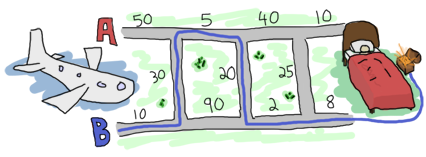
\includegraphics[width=0.7\textwidth]{road1_4.png}
\end{figure}

А знаете что ещё бы нам пригодилось?
Возможность запускать программу вне оболочки Erlang.
Опять слегка изменим нашу функцию main:
\begin{lstlisting}[style=erlang]
main([FileName]) ->
    {ok, Bin} = file:read_file(FileName),
    Map = parse_map(Bin),
    io:format("~p~n",[optimal_path(Map)]),
    erlang:halt().
\end{lstlisting}

Теперь арность функции main равна 1.
Это позволит нам получить параметры командной строки.
Я добавил вызов функции \ops{\href{http://erldocs.com/R15B/erts/erlang.html\#halt/0}{erlang:halt/0}}, после которого виртуальная машина Erlang завершает работу, и завернул вызов \ops{optimal\_path/1} в \ops{io:format/2}, потому что вне оболочки Erlang текст можно отобразить только таким способом.

С этими поправками файл \href{http://learnyousomeerlang.com/static/erlang/road.erl}{road.erl} примет следующий вид (не учитывая комментарии):
\begin{lstlisting}[style=erlang]
-module(road).
-compile(export_all).
 
main([FileName]) ->
    {ok, Bin} = file:read_file(FileName),
    Map = parse_map(Bin),
    io:format("~p~n",[optimal_path(Map)]),
    erlang:halt(0).
 
%% Transform a string into a readable map of triples
parse_map(Bin) when is_binary(Bin) ->
    parse_map(binary_to_list(Bin));
parse_map(Str) when is_list(Str) ->
    Values = [list_to_integer(X) || X <- string:tokens(Str,"\r\n\t ")],
    group_vals(Values, []).
 
group_vals([], Acc) ->
    lists:reverse(Acc);
group_vals([A,B,X|Rest], Acc) ->
    group_vals(Rest, [{A,B,X} | Acc]).
 
%% Picks the best of all paths, woo!
optimal_path(Map) ->
    {A,B} = lists:foldl(fun shortest_step/2, {{0,[]}, {0,[]}}, Map),
    {_Dist,Path} = if hd(element(2,A)) =/= {x,0} -> A;
                    hd(element(2,B)) =/= {x,0} -> B
                  end,
    lists:reverse(Path).
 
%% actual problem solving
%% change triples of the form {A,B,X}
%% where A,B,X are distances and a,b,x are possible paths
%% to the form {DistanceSum, PathList}.
shortest_step({A,B,X}, {{DistA,PathA}, {DistB,PathB}}) ->
    OptA1 = {DistA + A, [{a,A}|PathA]},
    OptA2 = {DistB + B + X, [{x,X}, {b,B}|PathB]},
    OptB1 = {DistB + B, [{b,B}|PathB]},
    OptB2 = {DistA + A + X, [{x,X}, {a,A}|PathA]},
    {erlang:min(OptA1, OptA2), erlang:min(OptB1, OptB2)}.
\end{lstlisting}

Исполним код:
\begin{lstlisting}[style=erlang]
$ erlc road.erl
$ erl -noshell -run road main road.txt
[{b,10},{x,30},{a,5},{x,20},{b,2},{b,8}]
\end{lstlisting}

Да, всё верно!
Для запуска программы больше ничего делать не нужно.
Эти две строки можно завернуть в единый bash/bat файл, или применить для этого \href{http://erlang.org/doc/man/escript.html}{escript}.

На примере этих двух упражнений мы увидели, что решать задачу становится проще, если сначала разбить её на мелкие части, по отдельности решить каждую подзадачу, а затем соединить всё воедино.
Мы также увидели, что нет смысла  начинать программирование до полного прояснения задачи.
Ну и несколько тестов, конечно же, никогда не будут лишними.
С их помощью вы убедитесь, что всё работает как положено и сможете менять код без изменения конечного результата.
